% --------------------------------------------------------------------

\section{Johdanto}

Tämä kandinaatintyö käsittelee eleentunnistusta Kinect-syvyyskameran avulla. 
Työn tarkoitus on tutustua erilaisiin eleentunnistusmenetelmiin ja erityisesti Chalearn Gesture Challenge -kilpailun kilpailutöihin. 
\\

Kuvaa ja videokuvaa on tutkittu paljon, mutta eleentunnistus on edelleen suuri haaste. Ihmisen eleet
ovat monimutkaisia ja niiden esitystapa vaihtelee esiintyjästä ja tilanteesta riippuen. Eleentunnistuksella
on kuitenkin monia käyttötarkoituksia esimerkiksi erilaisissa elekäyttöliittymissä. Toistaiseksi
eleentunnistusmenetelmät eivät ole olleet riittävän luotettavia ja nopeita, jotta niitä olisi voitu
laajasti hyödyntää kuluttujasovellukissa.\\

Kehittynyt tekniikka kuten Microsoftin Kinect-sensori ja kehittynyt laskentateho tuovat alalle uusia mahdollisuuksia. 
Kinect-sensori on Microsoftin kehittämä 3D-kamera, joka tarjoaa ns. 3D-videokuvaa eli tavallisen värikuvan lisäksi Kinect-kamera antaa infrapunakameralla mitattua syvyyskuvaa. 
3D-videokuvan avulla eleitä voidaan tunnistaa 2D-videokuvaa luotettavammin. 3D-kuva ei ole kuitenkaan 
vielä toistaiseksi radikaalisti kehittänyt tai muuttanut olemassa olevia eleentunnistusmenetelmiä.\\

Lisätäkseen kiinnostusta 3D-kuvaan järjestettiin ChaLearn Gesture Challenge -eleentunnistuskilpailu, joissa kilpailijat kehittivät Kinect sensorin datalle suunnattuja 
eleentunnistusmenetelmiä. Tämä kandinaatin työ tutustuu kilpailutöihin ja kartoittaa niiden avulla alan uusinta tutkimusta. Kilpailu on hyvä tutkimuskohde,
sillä sen avulla voidaan puolueettomasti vertailla erilaisia menetelmiä. Eleentunnistukselle on tyypillistä, 
että menetelmät oppivat liiankin hyvin opetusdatajoukkoon, eivätkä ole enää yleistettävissä muille datajoukkoille. Jotta saadaan vertailtavissa olevia tuloksia, on eri menetelmiä testattava samalla ja mielellään kokonaan uudella datajoukolla.\\

ChaLearn Gesture Challenge -kilpailussa jaettiin Kinect-sensorilla kuvattuja näytteitä erilaisista eleistä.
Jokaisesta eleestä annettiin yksi näyte, koska kilpailijoita haluttiin kannustaa kehittämään yhdestä 
eleestä oppimiseen sopivia menetelmiä (One Shot Learning). Tämä näkökulma näkyi kuitenkin kilpailutöissä
vähän. Kilpailutöiden menetelmät olivat pääasiallisesti sellaisia, että ne soveltuisivat myös tavalliselle
2D-videokuvalle. Menetelmät yhdistelivät tunnettuja menetelmiä kuvan, videon ja äänentunnistuksesta.\\

Luvussa kaksi esitellään vielä tarkemmin eleentunnistusongelmaa ja 3D-videokuvaa. Luvussa kolme kerrotaan
ChaLearn Gesture Challenge -kilpailusta ja luodaan yleiskatsaus kilpailutöihin. Luvussa neljä esitellään
tarkemmin kolme kilpailutöistä. Työ pyrkii kartoittamaan minkälaisia keinoja
3D-videokuvan tunnistuksessa voidaan käyttää ja miten 3D-kuvaa pystytään hyödyntämään eleentunnistuksessa.


\section{Eleentunnistus videokuvalta}
\label{eleentunnistus videokuvalta}


\subsection{Eleentunnistus ongelmana}
Eleentunnistuksella tarkoitetaan tässä työssä ihmisen suorittaman eleen tunnistamista videokuvalta. Eleitä voisivat olla esimerkiksi
viittomakielen eleet tai yksinkertaiset toiminnot kuten istuminen. Eleentunnistus on haastava ongelma. Ihmisen eleet ovat
monimutkaisia ja videokuvalla on paljon muuttujia kuten valaistus, tila tai kohteen etäisyys kamerasta.\citep {1251144} Luokan sisällä on paljon vaihtelua eli sama ele näyttää erilaiselta tilanteesta riippuen.
Yhtenä haasteena on ollutkin riittävän monipuolisen opetus- ja testitietokannan kerääminen
(HOG/HOF from movies). Syvyyskameroiden avulla ongelman ratkaisuun saadaan uusia työkaluja.\citep {6239178}\\

Eleentunnistus on hyvä erottaa asennontunnistus (Pose Estimation) -ongelmasta.
Asennontunnistuksessa pyritään tunnistamaan ihmisen asento videolla yhdessä pysäytyskuvassa
käyttämättä lainkaa ajallista tietoa. Ongelmana se on jossain määrin helpompi
kuin eleentunnistus, sillä hahmontunnistus kuvalta on yksinkertaisempaa kuin videokuvalta ja sitä on tutkittu enemmän. 
Yksittäisiä asentoja voidaan käyttää tunnistamaan ele, joskin se on laskennallisesti raskasta. (x-box artikkeli).   \\

Kiinnostus eleentunnistusta kohtaan on lisääntynyt viime vuosina sen monien käyttötarkoitusten vuoksi.
Eleentunnistusta voidaan käyttää monenlaisissa elekäyttöliittymissä. \citep {1251144} Yksittäisiä eleitä voidaan käyttää esimerkiksi kodinkoneiden ohjailuun. Toisaalta eleentunnistusta voidaan käyttää hyödyksi tunnistamaan
erilaisia vaaratilanteita. Esimerkiksi potilaan tilaa voidaan seurata eleentunnistuskameralla mahdollisten poikkeavien eleiden varalta.(chalearn toinen kierros)
\\

Videokuvan tunnistuksessa voidaan hyödyntää perinteisiä hahmontunnistusmenetelmiä. Monet menetelmistä ovat laskennallisti liian raskaita 
reaaliaikaseen videokuvan tunnistukseen. \citep {1251144} Monet hahmontunnistusmenetelmät vaativat myös paljon opetusdataa. Kuluttajille suunnatuissa
sovelluksissa olisi toivottavaa, että uuden eleen voi opettaa muutaman testinäytteen perusteella \citep {1251144}.\\

Eleentunnistuksessa, kuten hahmontunnistuksessa yleensä, pyritään matkimaan ihmisen toimintamalleja. Ihminen
kykenee oppimaan eleet yhden opetusnäytteen perusteella ja tunnistaa eleet tehokkaasti ulkoisista muuttujista riippumatta. 
Käytännössä huimaa vauhtia kehittynyt tekniikka on kuitenkin
viime aikoina ajanut tutkimuksen ohi ja monet menetelmät on kehitetty nopeasti lähinnä vastaamaan käytännön tarpeisiin ja tämä näkökulma on unohdettu. (Results and Analysis of the ChaLearn Gesture Challenge 2012)

\subsection{3D-videokuva}
Kinect-sensori on Microsoftin kehittämä kaupallinen 3D-kamera. (x-box artikkeli)
Tavallisen värikuvan lisäksi Kinect-sensori kuvaa infrapunakameran avulla syvyyskuvaa kohteesta.
Syvyyskuva kertoo kohteen etäisyyden kamerasta ja luo näin kolmiuloista videokuvaa. \\

Eleentunnistuksen näkökulmasta syvyyskuvalla on monia etuja verrattuna värikuvaan. Syvyyskuva on yksiväristä eli siitä on riisuttu erilaiset värit ja tekstuurit, jotka
usein aiheuttavat ongelmia värikuvan tunnistamisessa. Syvyyskuvan värisävyt on pakotettu tietylle 
asteikolle, mikä helpottaa kuvien vertailtavuutta. (x-box artikkeli) Hahmo on helposti erotettavissa
taustastaan ja eleet, jotka eroavat toisistaan ainostaan syvyysuuntaisen liikkeen perusteella, 
on mahdollista erottaa huomattavasti luotettavammin kuin pelkän värikuvan perusteella.\\

muita vastaavia kameroita? tarkempia speksiejä? mikrosofin politiikkaa

\subsection{Eleentunnistus video- ja 3D-videokuvalta}

Eleentunnistus videokuvalta noudattaa tavallisia hahmontunnistuksen vaiheita: esikäsittely, piirrevalinta ja
luokittely. Eleentunnistuksen erityishaasteet on huomioitava erityisesti piirrevalinnassa. 3D-videokuva tuo 
oman lisänsä, mutta se ei merkittävästi muuta työvaiheita. Eleentunnistus on hahmontunnistuksen termein
luokitusongelma eli mahdolliset luokat tunnetaan ennalta.(ensimmäinen chalearnartikkeli)  \\

Esikäsittelyssä vaiheessa videokuvalta pyritään poistamaan häiriötä, jotka voisivat haitata eleentunnistusta.
Näitä voivat olla esimerkiksi videokuvan virheet kuten kohina tai kuvassa esiintyvät ylimääräiset objektit.
Kuvaa voidaan myös pienentää tai pakata laskennan nopeuttamiseksi. Esikäsittelyssä pyritään usein myös erottamaan ihmishahmo taustasta. Tämä on haastavaa sillä
ihmishahmo ei välttämättä erotu esimerkiksi väritykseltään taustasta. Kinectin syvyyskameran avulla tämä onnistuu kuitenkin luotettavammin kuin pelkän 
värikuvan avulla. Ihmishahmon erottaminen taustasta helpottaa tunnistusta, sillä tällöin ihminen ei sekoitu taustaansa tai mitään taustassa olevaa
esinettä ei erehdytä pitämään ihmisen osana. Esikäsittelyssä voidaan suorittaa myös jonkinlaista ajallista jakoa tai tiivistystä. Videokuvaa
voidaan esimerkiksi jakaa ajallisiin jaksoihin perustuen videokuvan samankaltaisuuteen. Ajallisen jaon 
tarkoitus on auttaa hahmottamaan kuvalla tapahtuvaa liikesarjaa ja helpottaa tunnistusta. (ensimmäinen chalearn artikkeli)\\

Hahmontunnistuksessa ratkaiseva vaihe on usein oikeiden piirteiden valinta. Videokuvasta voidaan valita piirteeksi esimerkiksi 
tietyn suuntainen liike ajan funktiona. Liike näkyy peräkkäisten pysäytyskuvien välisenä erona. Tutkimalla liikettä
videokuvat voidaan tiivistää yksittäisiin liikekuviin, joita voidaan luokitella yksinkertaisilla 
luokittelualkoritmeillä. Videokuvasta voidaan tarkastella myös pysäytyskuvien kautta. Tällöin voidaan hyödyntää valokuvien tunnistustuksessa käytettyjä menetelmiä.
Pysäytyskuvista voidaan arvioida kontrastivaihteluita ja sitä kautta hahmottaa viivoja tai muotoja kuvassa.
Piirteisiin voidaan liittää myös ajallista rakennetta kuvaavaa informaatiota.
(ensimmäinen chalearn artikkeli). \\

Tunnistusvaiheessa annettuja näytteitä verrataan opetusdatan kuvaamiin luokkiin. Tunnistusmenetelmä riippuu valituista piirteistä.
Jos videokuvaa käsitellään kokonaisuutena esimerkiksi liikekuvan avulla, kuvia voidaan luokitella yksinkertaisilla luokittelu 
algoritmeillä. Näitä voisivat olla esimerkiksi k-lähimmän naapurin luokitin. Jos videokuva esitetään yksittäisillä pysäytyskuvilla 
on tunnistuksessa huomioitava videon aikaulottuvuus. On käytettävä rakenteellista mallia, jonka avulla voidaan tarkastella piirteen arvoa
tietyllä ajanhetkellä. Tässä voitaisiin käyttää esimerkiksi Markovin piilomallia \citep. \\

Luokittelun jälkeen menetelmälle lasketaan virheprosentti. Virheprosentti lasketaaan testidatan avulla.
Testidatassa on annettu näytteiden oikeat luokat, jolloin on mahdollista laskea, kuinka suuri prosentti
näytteistä on luokiteltu oikeisiin luokkiin. Menetelmää voidaan kehittää edelleen kokeilemalla erilaisia
opetusdatajoukkoja ja valitsemalla joukko, joka tuottaa pienimmän virheprosentin testidatalle. 

\section{ChaLearn Gesture Challenge -kilpailu}
\label{ChaLearn Gesture Challenge -kilpailu}

\subsection{Kilpailun esittely}
ChaLearn Gesture Challenge -kilpailun tarkoituksena oli lisätä kiinnostusta eletunnistukseen syvyyskameralla.
Kilpailu alkoi vuoden 2012 aikana ja se päättyi alkuvuonna 2013.
Kilpailussa tarjottiin tietokanta, joka sisälsi 50 000 Kinect-sensorilla kuvattua videonäytettä. Videonäytteet sisälsivät yksittäisiä
eleitä, esimerkiksi viittomia tai poliisin käsimerkkejä. Kilpailijoiden tarkoitus oli kehittää eleentunnistusmenetelmä, jonka avulla eleet
opitaan yhdestä opetusnäytteestä. Eleitä oli jaettu kategorioihin käyttötilanteen mukaan. Esimerksi poliisin käsimerkit olivat yksi kategoria. 
Eleet, joilla kilpailutöitä testattiin olivat eri eleitä kuin opetusdatassa, mutta samoista kategorioista.\\

Jokaisesta eleestä annettiin ainoastaan yksi opetusnäyte. Kilpailun erityishaasteena olikin One-Shot learning eli yhdestä otoksesta oppiminen. Tarkoituksena oli siis kehittää järjestelmä, joka oppii
tunnistamaan eleet mahdollisimman pienestä määrästä opetusdataa. Kilpailijoiden odotettiin soveltavan
tässä Transfer learning -menetelmää. eli ????\\

Annetuilla videonäytteillä esiintyi aina yksi ihminen kerrallaan suorittamassa tiettyä elettä. Kuva rajattiin yläruumiiseen ja eleet tehtiin
pääasiallisesti käsillä. Liikkeet lopetettiin ja aloitettiin aina samasta lepoasennosta. Videonäytteet sisälsivät syvyyskamerakuvan sekä värikuvan 
mutta eivät ranganseurausta. Haasteita toivat vaihtelevat taustat ja valaistukset videoilla. \\

Kilpailijoille jaettiin kolme datajoukkoa: opetusdata, validointidata ja lopullinen arviointidata.  Opetusdatan näytteille tarjottiin oikeat luokat, joiden avulla järjestelmän opetus onnistui.
Kilpailun loppupuolella paljastettiin lopullinen testidata, jonka avulla tuloksia arvioitiin.
\citep {6239178} \\


\subsection{Katsaus kilpailutöihin}
\subsubsection {Ensimmäinen kierros}
Kilpailijoiden metodeja selvitettiin ensimmäisen kierroksen jälkeen lyhyellä kyselyllä, johon vastasi 20 ryhmää 22 parhaan ryhmän joukosta.
Ryhmiltä kysyttiin muun muassa minkälaista esikäsittelyä he olivat tehneet videokuvalle, minkälaista tunnistusmenetelmää oli käytetty ja
mikä oli heidän menetelmänsä suoritusaika. Kyselyn tarkoituksena oli saada yleiskatsaus kilpailutöihin, sillä monet kilpailijat
halunneet julkaista yksityiskohtaista kuvausta menetelmästään kilpalun ollessa vielä kesken. \citep {6239178}. \\

Vastauksista kävi ilmi, että lähes kaikki ryhmät tekivät jonkinlaista kuvan esikäsittelyä. Videokuvasta poistetiin häiriötä, asiaanliittymättömiä 
kohteita tai ihmishahmon tausta. Huomioitavaa on kuitenkin, että jotkin hyvin menestyneistä ryhmistä eivät tehneet minkäänlaista esikäsittelyä kuvalle.
\citep {6239178}\\

Suurin osa osallistujista käytti piirteinä HOG/HOF-piirteitä (Histogram of oriented Gradients/ Histogram of Flow), SIFT/STIP-piirteitä (Scale Invariant Feature Transformation), 
kulmien tai nurkkien tunnistusta tai kehitti omia, tälle datalle soveltuvia piirteitä.\\

Käytetyt piirteet perustuvat pääosin kuvan värityksen intensiteettivaihteluun.
HOG -piirteet kuvaavat kuvan intensitettivaihtelun gradienttien suuntaa. Kuva jaetaan pieniin alueisiin, soluihin, 
joissa tarkastellaan alueen värityksen intensiteettivaihtelua. Soluille lasketaan intensiteettivaihtelun gradienttien suuntien histogrammi. 
Ajatuksena on päätellä, minkä suuntaisia viivoja tai nurkkia alueelta voidaan erottaa.\citep {1467360} Histogrammit kertovat kuvassa esiintyvistä
muodoista, eivätkä ne ole riippuvaisia hahmon sijainnista kuvassa tai kuvan yleisestä värimaailmasta.
HOG-piirteet soveltuvatkin hyvin tämänkaltaiseen hahmontunnistusongelmaan, jossa kohteen sijainti voi vaihdella kuvalla.\\

SIFT-piirteet toimivat HOG-piirteitä hienostuneemmin valiten kuvista tärkeät pisteet. Tärkeät pisteet valitaan niin, että ne ovat riippumattomia
kuvan muutoksista kuten kiertämisestä tai skaalauksesta. \citep {790410} Esimerkiksi kuvassa, jossa näkyy ovi, tärkeitä pisteitä voisivat olla oven kulmat.
Vaikka kuvaa kierrettäisiin tai sen kokoa muutettaisiin, tärkeät pisteet eli kulmat voidaan löytää kuvasta.
Pisteiden valinnassa hyödynnetään värityksen intensiteettivaihtelua ja tilastolllisia menetelmiä. \\

Piirteitä voidaan tutkia syvyys- ja värikuvasta. Syvyyskuvan etu verrattuna värikuvaan on, että siinä
ei esiinny värejä tai tekstuureja, jotka häiritsisivät hahmon erottumista tai videoiden vertailua.
Suurin osa kilpailijoista käyttikin töissään pelkkää syvyyskuvaa. Osa käytti sekä väri- että syvyyskuvaa. 
Mielenkiintoista on, että ensimmäisen kierroksen toisen sijan voittaja käytti työssään pelkkää värikuvaa. 
Kaikki kilpailijat käyttivät jonkilaista piirteiden tiivistystä tai kuvausta toiseen lineaariavaruuteen.\\ 

Ajallisen rakenteen mallintamiseen käytettiin erilaisia graafisia malleja kuten Markovin piilomuuttujaa ja Conditional Random Fields-menetelmää. Kaikki tunnistustusmenetelmät eivät huomioineet videon ajallista rakennetta ollenkaan.\\

Markovin muuttuja kuvaa havainnon sarjana tiloja eli tässä tapauksessa videon sarjana pysäytyskuvia. Menetelmä kertoo kuinka todennäköisesti annettu havainto 
kuuluu tiettyn luokkaan. Ajatuksena on, että annetun havainnon luokka on tuntematon, mutta voimme löytää sen etsimällä todennäköisimmän luokan. 
Ajatellaan, havainto koostuu peräkkäisistä tiloista eli tässä tapauksessa kuvista, jotka voidaan esittää ennalta sovittujen piirteiden avulla.
Havainnon tiloja verrataan ennalta opittujen luokkien tilojen kanssa ja valitaan se luokka, mihin havainto todennöisimmin kuuluu. Luokkien tiheysfunktiot
lasketaan suurimman todennäköisyyden (Most Likelihood) -menetelmällä. Kyseessä on Bayesialainen menetelmä, jakauma tunnetaan, mutta ei parametreja.
Parametrien arvot optimoidaan niin, että todennäköisyys opetusliikkeelle kuulua kuvaamaansa luokkaan on mahdollisimman suuri. Luokkien tiheysfunktioiden
avulla lasketaan, kuinka todennäköisesti annettu havainto kuuluu tiettyyn luokkaan.\citep {}  \\

Conditional Random Fields -menetelmä perustuu samankaltaiseen logiikkaan. \citep {} Lähtökohta molemmissa on, että yksittäisen 
datapisteen sijaan luokitellaan datajoukkoja, joilla on sisäinen, tässä ajallinen, rakenne. \\

Itse luokittelu tapahtui k-lähimmän naapurin luokittimella tai muilla yksinkertaisilla luokittelumenetelmillä. 
Kilpailun järjestäjien odottamaa metodia Transfer learning -metodia käytettiin vähäisesti, eikä kukaan menestyneistä kilpailijoista käyttänyt sitä.
Kilpailun varsinainen haaste, yhdestä eleestä oppiminen, jäi siis vähemmälle huomiolle. \citep {6239178} \\

Kahdeksan menestyneintä työtä esitellään taulukossa ~\ref{table:dvbt_param}. Taulukosta huomataan, että parhaiten menestyneiden töiden
joukossa suurin osa käytti tunnistukssa menetelmää, joka huomioi videon ajallisen rakenteen. Videokuvasta valitaan piirteet esimerkiksi HOG-piirteet, joiden
muutosta seurataan ajan funktiona. Poikkeuksen tekevät ryhmät Zonga ja Xiaozhuwudi, joiden menetelmä perustuu videon käsittelyyn erilaisten liikekuvien avulla. 

\begin{table}[th]
\caption{ChaLearn Challenge kahdeksan parhaiten sijoittunutta ryhmää}
\label{table:dvbt_param}
\begin{center}
\begin{tabular}{|p{0.35\textwidth}|p{0.45\textwidth}|} 
    \hline
Ryhmän nimi & Menetelmä \\
    \hline
    \hline
Alfnie & Motion Signature analyses\\ 
    \hline
Pennect & Markovin piilomallin tapainen menetelmä ja HOG/HOF-piirteet.\\
    \hline
One Million Monkeys & Markovin piilomalli ja kulmien tunnisus\\
    \hline
Immortals & Markovin piilomalli ja HOG/HOF-piirteet\\
    \hline
Zonga & Pienimmänneliösumman menetelmä ja HOSVD -menetelmä\\
    \hline
Balazs Godeny & Thumbnail Dynamic Time Warping” (DTW) ja HOG/HOF-piirteet sekä kulmien tunnistus.\\
    \hline
SkyNet & Dynamic Time Warping(DTW) ja kulmien tunnistus\\
    \hline
Xiaozhuwudi & MHI-kuva johon on lisätty GEI- ja INV-kuvat\\
    \hline	
\end{tabular}
\end{center}
\end{table}

Luvussa kaksi esitellään kolme menestyneistä töistä tarkemmin. Työt ovat eräitä esimerkkejä toimivista ratkaisuista. Ne on valittu tähän, 
koska ne edustavat erilaisia näkökulmia ongelmaan. Valintamahdollisuuksia rajoitti se, että kaikki kilpailijat eivät olleet vielä julkaisseet 
menetelmäänsä tämä työn kirjoittamisen aikana. Kolmesta valitusta työstä yksi, Immortals edustaa kilpailun yleislinjaa ja kaksi muuta valittua työtä,
Zonga ja Xiaozhuwudi ovat esimerkkeinä omaperäisemmistä menetelmistä.\\

\subsubsection {Toinen kierros}

Kilpailun toinen kierros toteutettiin samoilla järjestelyillä kuin ensimmäinen. Koska kierros loppui
vasta tämän kandinaatintyön kirjoittamisen aikoihin, on se jätetty työssä vähemmälle tarkastelulle.\\

Toisen kierroksen jälkeen kilpailijoiden metodeja selvitettiin kyselyllä samoin kuin ensimmäisen
kierroksen jälkeen. Kyselyyn vastasi 28 ryhmää. Vastausten perusteella toisella kierroksella menestyneet 
menetelmät olivat hyvin samantapaisia kuin ensimmäisen kierroksen menestyneet menetelmät. HOG/HOG-piirteet sekä muut
kuvan intensiteettivaihteluihin perustuvat piirteet yhdistettynä Markovin piilomuuttujaan tai muuhun
vastaavaan malliin olivat suosituin menetelmä.\\

Molemmilla kierroksilla oli sama voittaja, ryhmä Alfnie. 
Voittajaryhmä väittää työnsä matkivan ihmisen hahmontunnistuskykyä. Työtä ei ole kuitenkaan vielä tämän kandinaatintyön kirjoittamisen aikaan julkaistu, joten siihen ei päästä tutustumaan tarkemmin. Työ perustuu
ryhmän ilmoituksen mukaan jonkinlaiseen kustomoituun Markovin piilomuuttujaan. Mielenkiintoista on,
että huolimatta hyvästä sijoituksestaan meneltemä oli myös yksi kilpailun nopeimmista.\\

Toisen sijan voittaja toisella kierroksella, ryhmä Turtle Tamers, käytti samankaltaista menetelmää kuin 
ensimmäisen kierroksen toisen sijan voittaja, ryhmä Pennect. Molemmat ryhmät käyttivät HOG/HOF-piirteitä sekä Markovin piilomallia. 
Kolmannen sijan saavuttanut ryhmä Joewan sen sijaan käytti hyvin erilaista menetelmää. Ryhmä käytti Bag of MOSIFT -
piirteitä yhdistettynä lähimmän naaprin luokittimeen. Bag of MOSIFT -piirteet on kustoimoitu versio
yleisestä Bag of features -menetelmästä. Bag of features -menetelmät kuvaavat kuinka usein tietty 
arvo esiintyy näytteessä. Ne hajottavat näytteen sisäisen rakenteen ja eroavat siis Markovin piilomallista,
joka säilyttää näytteen sisäisen rakenteen \citep{}. \\

Varsinaisen validoinnin lisäksi kilpailutöille suoritettiin vielä yksi testaus. Tässä testauksessa tutkittiin kuinka 
hyvin kilpailijoiden menetelmät tunnistivat eleen, jos videokuvaa oli tietoisesti käännetty hieman. Oikeissa sovelluksissa on tärkeää,
että ele pystytään tunnistamaan, vaikka se eroaisi hieman alkuperäisestä näytteestä esimerkiksi kuvakulmaltaan. 
Tässäkin testissä voittajaryhmä pärjäsi hyvin, kun taas esimerkiksi kaksi seuraavaa ryhmää pärjäsit manipuloidulla datalla huomattavasti
huonommin kuin varsinaisella kilpailudatalla. Tämä lisää ennestään mielenkiintoa voittajatyötä kohtaan.



\section {Katsaus menestyneisiin kilpailutöihin}

\subsection{Xiaozhuwudi ja laajennettu MHI-menetelmä}
Ryhmä xiaozhuwudi lähti liikkeelle MHI eli Motion History Image -tekniikasta. \citep {6239179} MHI tutkii liikkeen määrää videokuvalla.
Videopätkä tiivistetään yhteen liikekuvaan, joka kuvaa liikkeen viimeaikaisuutta. Kohdat, joissa videokuvalla on ollut
liikettä esitetään harmaasävyillä. Mitä viimeaikasempaa liike on ollut sitä valkoisempana se näkyy kuvassa. Liikkumattomat
alueet näkyvät täysin mustana. Videokuvalta tutkitaan siis vain liikettä, eikä pyritä esimerkiksi tunnistamaan kuvalla olevia kohteita
tai ihmiskehon osia. Tämä menetelmä matkii ihmisen tapaa tunnistaa eleitä. Ihminen tunnistaa erittäin hyvin inhimilliset eleet  
sumealtakin videokuvalta vaikka ei yksittäisestä framesta tunnistaisi edes ihmishahmoa. \citep {910878}  \\

\begin{figure}[htb]
  \begin{center}
    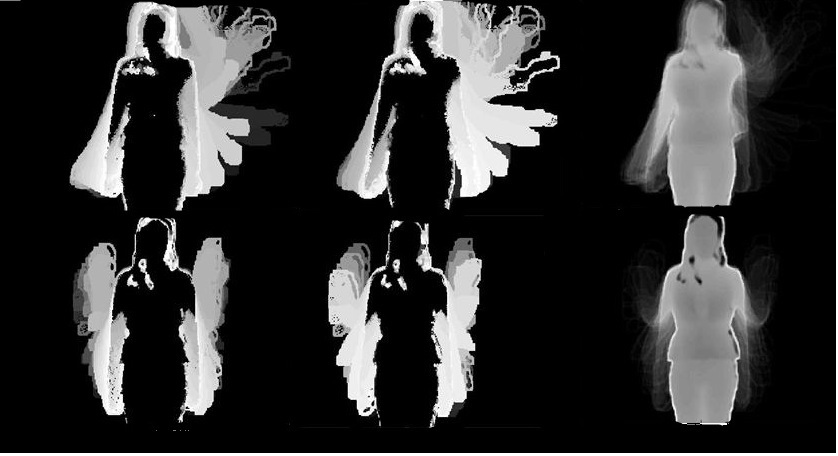
\includegraphics[width=0.9\textwidth]{mhi_ex.jpg}
    \caption{Kuvassa vasemmalta oikealle MHI, INV ja MEI. \citep {6239179}}
    \label{fig:mhiinvmei}
  \end{center}
\end{figure}

Xiaozhuwudi-ryhmä tunnistaa MHI:ssa kuitenkin ongelmia. MHI ei tunnista kovin hyvin eleitä, jotka sisältävät toistuvaa liikkeitä esimerkiksi vilkutusta.
Liikkeen toistuessa MHI -kuva muuttuu helposti sekavaksi ja on vaikea erottaa tarkkaa liikerataa. Xiaozhuwudi ehdottaa MHI:n laajentamista INV ja GEI -kuvilla.
INV oon käänteinen kuvaus MHI:ille. INV:ssa katsotaan videokuvaa alusta loppuun päin.
Mitä aikasemmin liike esiintyy videolla sitä vaalempana se näytetään kuvassa. INV:n avulla saadaan kuvaus videon alkutilanteesta, mikä täydentää MHI kuvaa. 
GEI-kuva esittäää liikkeen määrää keskimäärin koko videon aikana. Siinä summataan koko videon liike yhdelle kuvalle ja jaetaan lopuksi koko aikavälille.
GEI muistuttaa MEI:tä (Motion Energy Image), jossa myös lasketaan liikkeelle summa. Voidaan ajatella että siinä missä MHI ja INV mittaavat liikettä 
MEI ja GEI mittaavat energiaa, joka on kulunut liikkeeseen. GEI:n avulla liikkeestä saadaan hyvä kokonaiskuva ja se on hyödyllinen etenkin toistuvan
liikkeen tunnistuksessa. \citep {6239179} \\

Kuvassa ~\ref{fig:mhiinvmei} on esitetty kahdelle
liikkeelle MHI-, INV- ja GEI-kuvat. Kuvat havainnollistavat hyvin miten INV- ja GEI-kuvat
täydentävät MHI-kuvaa. Pelkän MHI-kuvan perusteella on vaikea erottaa liikkeet toisistaan.
INV- ja GEI-kuvien avulla liikkeet erottuvat kuitenkin selkeämmin. \\

Datan esikäsittelyssä xiaozhuwudi hyödynsi Kinectin syvyyskuvaa poistamalla taustan ihmishahmolta. Lisäksi esikäsittelyssä poistettiin häiriöitä.
MHI, GEI ja INV -kuville suoritettiin dimensioiden vähennys. Eleiden tunnistukseen käytettiin Maximum Correlation Coeffient -luokittelijaa. \citep {6239179}\\



\subsection{Immortals ja Markovin piilomalli}

Ryhmä Immortals esittää kilpailutyössään oletuksen, että ele koostuu ennen kaikkia useista yksittäisistä liikkeistä. 
Sen mukaan eleet tunnistetaan parhaiten käsittelmällä elettä sarjana liikkeitä. Tämä eroaa ryhmän mukaan tyypillisestä 
tavasta lähestyä ongelmaa.\\

Ryhmä lähti liikkeelle opetusvaiheessa yksittäisistä liikkeistä. Yksittäisille liikkeille luodaan allekirjoitus eli malli,
jonka avulla ne voidaan tunnistaa. Allekirjoituksen luominen on monivaiheinen operaatio. Ensin kuvista poimitaan niin sanotut
tärkeät pisteet eli pisteet joilla on merkitystä liikkeen tunnistamisen kannalta. Tässä Immortals hyödynsi Kinectin syvyyskuvaa.
Immortals arvioi, että ne kohdat kuvasta joissa on tapahtunut syvyyssuuntaista muutosta syvyyskameran kuvassa ovat kyseisen videon pysäytyskuvan
tärkeitä pisteitä. Tärkeille pisteille lasketaan HOG (Histogram of oriented gradients) ja HOF (Histogram of Flow). 
Tämän jälkeen kaikkien kuvien kaikki histogrammit ryhmitellään tavallisen ryhmittelyalgoritmin avulla.
Histogrammeja kutsutaan ryhmittelyn jälkeen "visuaalisiksi sanoiksi". Yhdessä ryhmässä ovat kaikki tietyn sanan esiintymät.
Tarkoituksena on tutkia visuaalisten sanojen esiintymistä yhdessä ja muodostaa niistä aihepiirejä. 
Yksittäistä pysäytyskuvaa voidaan kuvata sillä, mitä sanoja ja mistä aihepiireistä siinä esiintyy.\\

Liikkeelle luodaan sanojen perusteella perusteella malli, jota käytetään tunnistusvaiheesa. Mallin perustana on Markovin muuttuja
eli HMM (Hidden Markov Model). Koska tutkitaan kahta piirrettä, HOG- ja HOF-piirrettä, käytetään monikanavaista Markovin piilomallia eli McHMM. 
HOG- ja HOF-piirteet paljastavat erilaista tietoa havainnosta ja tukevat tässä hyvin toisiaan. McHMM parametreja ovat alkutila, 
todennäköisyys tilojen väliselle muutokselle sekä tilan todennäköisyys ja tilan kuvaus HOG ja HOF-piirteiden avulla. 
Tilalla tarkoitetaan tässä yksittäistä pysäytyskuvaa. Malli opetetaan parametrien avulla niin, että se tunnistaa tietyn liikkeen. \\

Tunnistusongelma pelkistyy lopulta kysymykseen: Mikä liikesarja kaikken todennäköisimmin on muodostanut tämän videonäytteen?
Tämän tyylinen ongelma voidaan ratkaista Viterbin algoritmillä. Tämä vaatii kuitenkin, että ele rajataan koostumaan tietystä määrästä liikkeitä.
Kilpailussa on määritelty, että jokainen elenäyte sisältää viisi liikettä.
Viterbin alkorytmi pyrkii löytämään todennököismmän polun eri liikkeiden välillä. Alkorytmi käy videota läpi liike kerrallaan ja laskee mikä
on mallien perusteella todennäköisin liike. Lopuksi saadaan liikesarja, josta videonäyte todennäköisimmin koostuu.
Liikesarja liitetään tunnistusvaiheessa tiettyyn eleeseen. \citep {6239185}\\ 


\subsection{Zonga ja pieninimmän neliösumman menetelmä sovelluttuna monistoon}
Ryhmä Zonga käyttää kehittämäänsä menetelmää, joka soveltuu yleisesti videokuvan luokitteluun. 
Menetelmää on kuitenkin kustomoitu eleentunnistusta varten tähän haasteeseen.\\

Videonkuvan käsittelyssä ensimmäinen tehtävä on usein kuvata videokuva vektoriksi tai tensoriksi, joka voidaan esittää tila-avaruudessa. 
Videokuva ei ole lähtökohtaisesti piste Euklidisessa avaruudessa, vaan monimuotoinen datajoukko. Datan käsittelymenetelmillä, kuten dimensioiden pienennyksellä, video saadaan kuitenkin kuvattua yksittäiseksi pisteeksi tila-avaruudessa. Avaruudessa olevia pisteitä voidaan käsitellä
ja esimerkiksi luokitella yksinkertaisten algoritmien avulla.\\

Ryhmä Zonga ehdottaa videon kuvamista pisteenä Grassmannin monistossa. Videokuvan kolme ulottuvuutta (leveys, korkeus ja aika) ovat moniston ulottuvuudet. 
Monisto säilyttää alkuperäisen havainnon geometrisen rakenteen paremmin kuin Euklidinen avaruus.
Havainnon alkuperäinen rakenne usein kadotetaan muissa eleentunnistusmenetelmissä. Monistojen käyttäminen ei ole uusi asia eletunnistuksessa, mutta
ryhmä Zonga yhdistää monistoihin pienimmän neliösumman menetelmän, mikä tekee ryhmän tekniikasta ainutlaatuisen. \\

Videokuvasta on helposti erotettavissa kolme ulottovuutta: leveys, korkeus ja aika. Tämän takia videokuvaa on luonnollista käsitellä sitä kolmiulotteisessa monistossa.
Pienimmän neliösumman menetelmä on regressio-ongelma, eli siinä etsitään jonkinlaista suhdetta havainnon ja luokan välille. Opetusvaiheessa tunnetaan havainto ja sen luokka, joiden väälille pyritään löytämään
funktio. Tunnistusvaiheessa luokat haavaintojen luokat lasketaan regressiofunktion avaulla.\\

Regressio-ongelma on tyypillisesti muotoa y = A * beta, jossa y -vektori esittää pisteet tulosavaruudessa, A on havaintomatriisi 
ja b -vektori on painovektori, joka kuvaa havaintomatriisin pisteet tulospisteiksi.
Opetusvaiheessa pyritään löytämään painovektori, joka kuvaa havainnon mahdollisimman lähelle oikeaa luokkaa
tulosavaruudessa. Pienimmän neliösumman menetelmässä pyritään minimoimaan luokitteluvirheen neliötä eli oikean tulokset ja arvioidun tuloksen erotuksen neliötä.
Minimoidaan siis funktiota: \\
R(beta) = ||y-A*beta|| \\
jolloin b:lle saadaan funktio\\
funktio tähän\\

Havaintomatriisi A muodostetaan kolmesta tekijästä: videon korkeussuuntaisesta kuvaajasta, leveyssuuntaisesta sekä ajallisesta vaihtelusta.
Havaintomatriisin luomisessa käytetään HOSVD:ia. Painovektori b kuvaa havaintomatriisin A tulosavaruuteen, missä kadotetaan tieto alkuperäisistä moinston tekijöistä. 
Lopullista luokittelua varten halutaan kuitenkin palauttaa pisteet monistoon.
Näin luokittelussa huomioidaan alkuperäisen havainnon rakenne. 
Lopullinen regressiokaava on siis muotoa\\
tähän se lopullinen kaava pisteen kera\\
Pistefunktio on operaatio joka kuvaa havainnot monistossa. Grasmanin monisto parametrisoi jokaisen vektoriavaruuden aliavaruuden.
Tässä tapauksessa parametreja on kolme, jokaiselle havainnon tekijälle.
Zonga suorittaa kuvauksen Karcher -keskiarvomenetelmää muistuttavalla menetelmällä.\\

Tunnistus tapahtuu vertaamalla kuvaamalla annetut pisteet monistoon ja vertaamalla niitä luokkiin etäisyyden avulla. \citep {6239180}\\


\subsection{Yhteenveto menestyneistä kilpailutöistä}
Menestyneet kilpailutyöt lähestyivät ongelmaa varsin erilaisin menetelmin ja panostivat eri vaiheesiin eleentunnistuksessa.\\
 
Ryhmä Xiaozhuwudi käytti työssään laajennettua MHI-kuvaa eli tutki videolla tapahtuvaa liikettä ohittaen yksittäiset pysäytyskuvat ja videon ajallisen rakenteen.
Ryhmä Zonga valitsi piirteiksi horisontaalisen ja vertikaalisen liikkeen videolla sekä kuvan "summan" videon yli. 
Ryhmä immortals sen sijaan lähti tutkimaan yksittäisiä pysäytyskuvia ja tutki kuvista muotoja HOG ja HOF -piirteiden avulla.\\

Tunnistusmenetelmät heijastelivat ryhmien piirrevalintoja. Xiaozhuwudi ja Zonga, jotka tiivistivät näytteet 
yksittäisiin kuviin käyttivät luokittelumenetelmiä, jotka perustuvat etäisyyden laskemiseen 
euklidissa tai sen kaltaisessa tilassa. \\

Immortals lähti oletuksesta, että videokuva koostuu ennen kaikkea joukosta perättäisiä yksittäisiä liikkeitä.
Markovin piilomallin avulla kuvattiin liikkeiden ajallinen rakenne. Luokittelussa pyrittiin löytämään 
liikesarja, joka kaikken todenäköisimmin esiintyi videolla. Ryhmän Immortals menetelmä edusti kilpailutöiden yleistä suuntausta.\\

Immortals sijoittui kilpailussa viidenneksi, Zonga kuudenneksi ja Xiaozhuwudi kahdeksanneksi. Parhaiten menestyneen Immortalssin
menetelmä vaikuttaa raskaimmalta, mutta ilmoituksen perusteella se on vain lineaarinen suhteessa opetusnäytteiden määrään.
Muut ryhmät ilmoittivat samankaltaisia lukemia.


\section {Johtopäätökset}

Kilpailutöiden perusteella 3D-videokuvan tunnistuksessa käytetään pitkälti samoja keinoja kuin 2D-videokuvan tunnistuksessa. Kilpailutyöt eivät huomioineet
3D-kuvaa erityisesti piirrevalinnassa tai tunnistusmentelmissä tai ainakaan tätä näkökulmaa ei tuotu erityisesti
esille kilpailutöiden kuvauksissa. 3D-videokuvaa hyödynnettiin esikäsittelyvaiheessa taustan irroittamiseen 
(lähes kaikki kilpailutyöt) ja ainakin yhdessä työssä (Immortals) tärkeiden pisteiden valinnassa. 
Lähes kaikki kilpailijat toki käyttivät syvyyskuvaa, osa jopa pelkästään sitä, mutta eivät juurikaan
kuvailleet miten heidän menetelmänsä olisi eronnut, jos käytössä olisi ollut pelkästään värikuva.
Kuvaavaa on, että kilpailussa toiseksi tullut työ hyödynsi pelkkää värikuvaa.\\

Kilpailijoiden käyttämistä menetelmistä lähes kaikki perustuivat ajallisen rakenteen mallintamiseen 
Markovin piilomuuttujan tai muun vastaavan menetelmän avulla. Piirteinä käytettiin erilaisia kuvan intensiteettivaihteeluun perustuvia piirteitä. Erityisiä perusteluita tälle ei kuitenkaan esitetty.
Kilpailussa menestyi hyvin myös muutama työ, jotka käyttivät täysin tästä poikkeavia menetelmiä.\\

Jatkotutkimuksen kannalta olisi mielenkiintoista selvittää kuinka hyvin kilpailutyöt pärjäisivät
muulle kuin tässä kilpailussa annetulle datalle. Toisen kierroksen kilpailutöiden tuloksissa oli viitteitä
siitä, että menetelmät olivat "ylioppineet" tälle datalle.(Chalearn2) Silloin ne tuottavat hyviä tuloksia juuri
tälle datalle, mutta eivät menestyisi yhtä hyvin muille datajoukoille. Esimerkiksi näytteille, jotka on esimerkiksi kuvattu kauempaa 
kohteesta tai jollain muulla tapaa eroavat tästä datasta. \\

Olisi mielenkiintoista tutustua myös voittajatyöhön, joskaan sen käyttämät menetelmät eivät pinnallisen
kuvauksen perusteella juuri eronneet kilpailun yleisestä suuntauksesta.




































% --------------------------------------------------------------------

\section{Loppuluku}



% --------------------------------------------------------------------

